% Nallino, Part I p. 250: Schiaparelli's figure of the epicycle, redrawn from the print: the circle about the
% Earth T through the centre O of the epicycle, the epicycle about O, the line from T through O to M, the tangents
% from T touching the epicycle at K and I, drawn on beyond them, the radii OK and OI, and the bold italic letters.
% Measured on the scan (_intake/latin/tools/fig250).
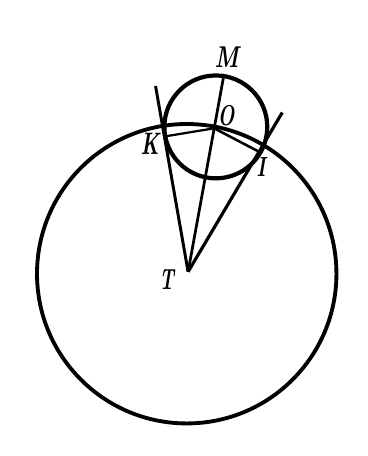
\begin{tikzpicture}[x=0.9892pt,y=-0.9892pt,line cap=butt,every node/.style={font=\fontsize{11}{11}\bfseries\itshape\selectfont,inner sep=0pt}]
\useasboundingbox (0,0) rectangle (114.00,146.00);
\draw[line width=1.39pt] (58.10,89.88) circle[radius=54.69];  % the circle about T
\draw[line width=1.52pt] (68.73,36.25) circle[radius=18.79];  % the epicycle about O
\draw[line width=0.99pt] (58.60,89.16) -- (71.74,16.94);  % the line from T through O to M
\draw[line width=1.07pt] (58.60,89.16) -- (46.71,21.32);  % the tangent TK, drawn on beyond K
\draw[line width=1.15pt] (58.60,89.16) -- (93.01,30.98);  % the tangent TI, drawn on beyond I
\draw[line width=0.81pt] (68.14,36.76) -- (49.96,39.75);  % the radius OK
\draw[line width=0.92pt] (68.14,36.76) -- (84.54,45.33);  % the radius OI
\node at (72.71,10.86) {\normalfont\fontsize{11}{11}\bfseries\itshape\selectfont \resizebox{8.69pt}{7.46pt}{M}};
\node at (72.43,32.18) {\normalfont\fontsize{11}{11}\bfseries\itshape\selectfont \resizebox{6.06pt}{7.11pt}{O}};
\node at (44.61,42.28) {\normalfont\fontsize{11}{11}\bfseries\itshape\selectfont \resizebox{6.70pt}{7.69pt}{K}};
\node at (85.26,50.72) {\normalfont\fontsize{11}{11}\bfseries\itshape\selectfont \resizebox{3.24pt}{6.86pt}{I}};
\node at (50.79,91.84) {\normalfont\fontsize{11}{11}\bfseries\itshape\selectfont \resizebox{5.29pt}{7.23pt}{T}};
\end{tikzpicture}
